Normalisers:

A normaliser is a class responsible with taking a packet and returning a ``normalised'' value of a certain attribute of that packet and the other way around. 
Each normalising class is able to create a temporary filter in the application that will filter its corresponding attribute on a certain range. 
Since the normalising class is in control of its filter it creates a zooming effect based on the range of the filter: the lower bound is normalised to 0, the upper bound to 1. 

Flow of Data through the application:
The data feeder creates Packet objects based on the traffic in analyses and feeds it to the Data Controller. 
We implemented a CSV data feeder that reads CSV files (/* maybe here a little more about the structure of the CSV's? */) created with Wireshark but the simple interface of the data feeder makes it easy to extend the application for reading live data.

The Data Controller uses the listener pattern and feeds new packets as they arrive to its listeners (visualizations, analysis panel).
If there are any active filters then the data controller will apply those filters to the data and supply only what is relevant.

When a filter is applied or changed a reset signal is sent from the data controller informing the visualizations that all the data has changed. Along with this signal a list of all the past packets (with filters applied) is provided.

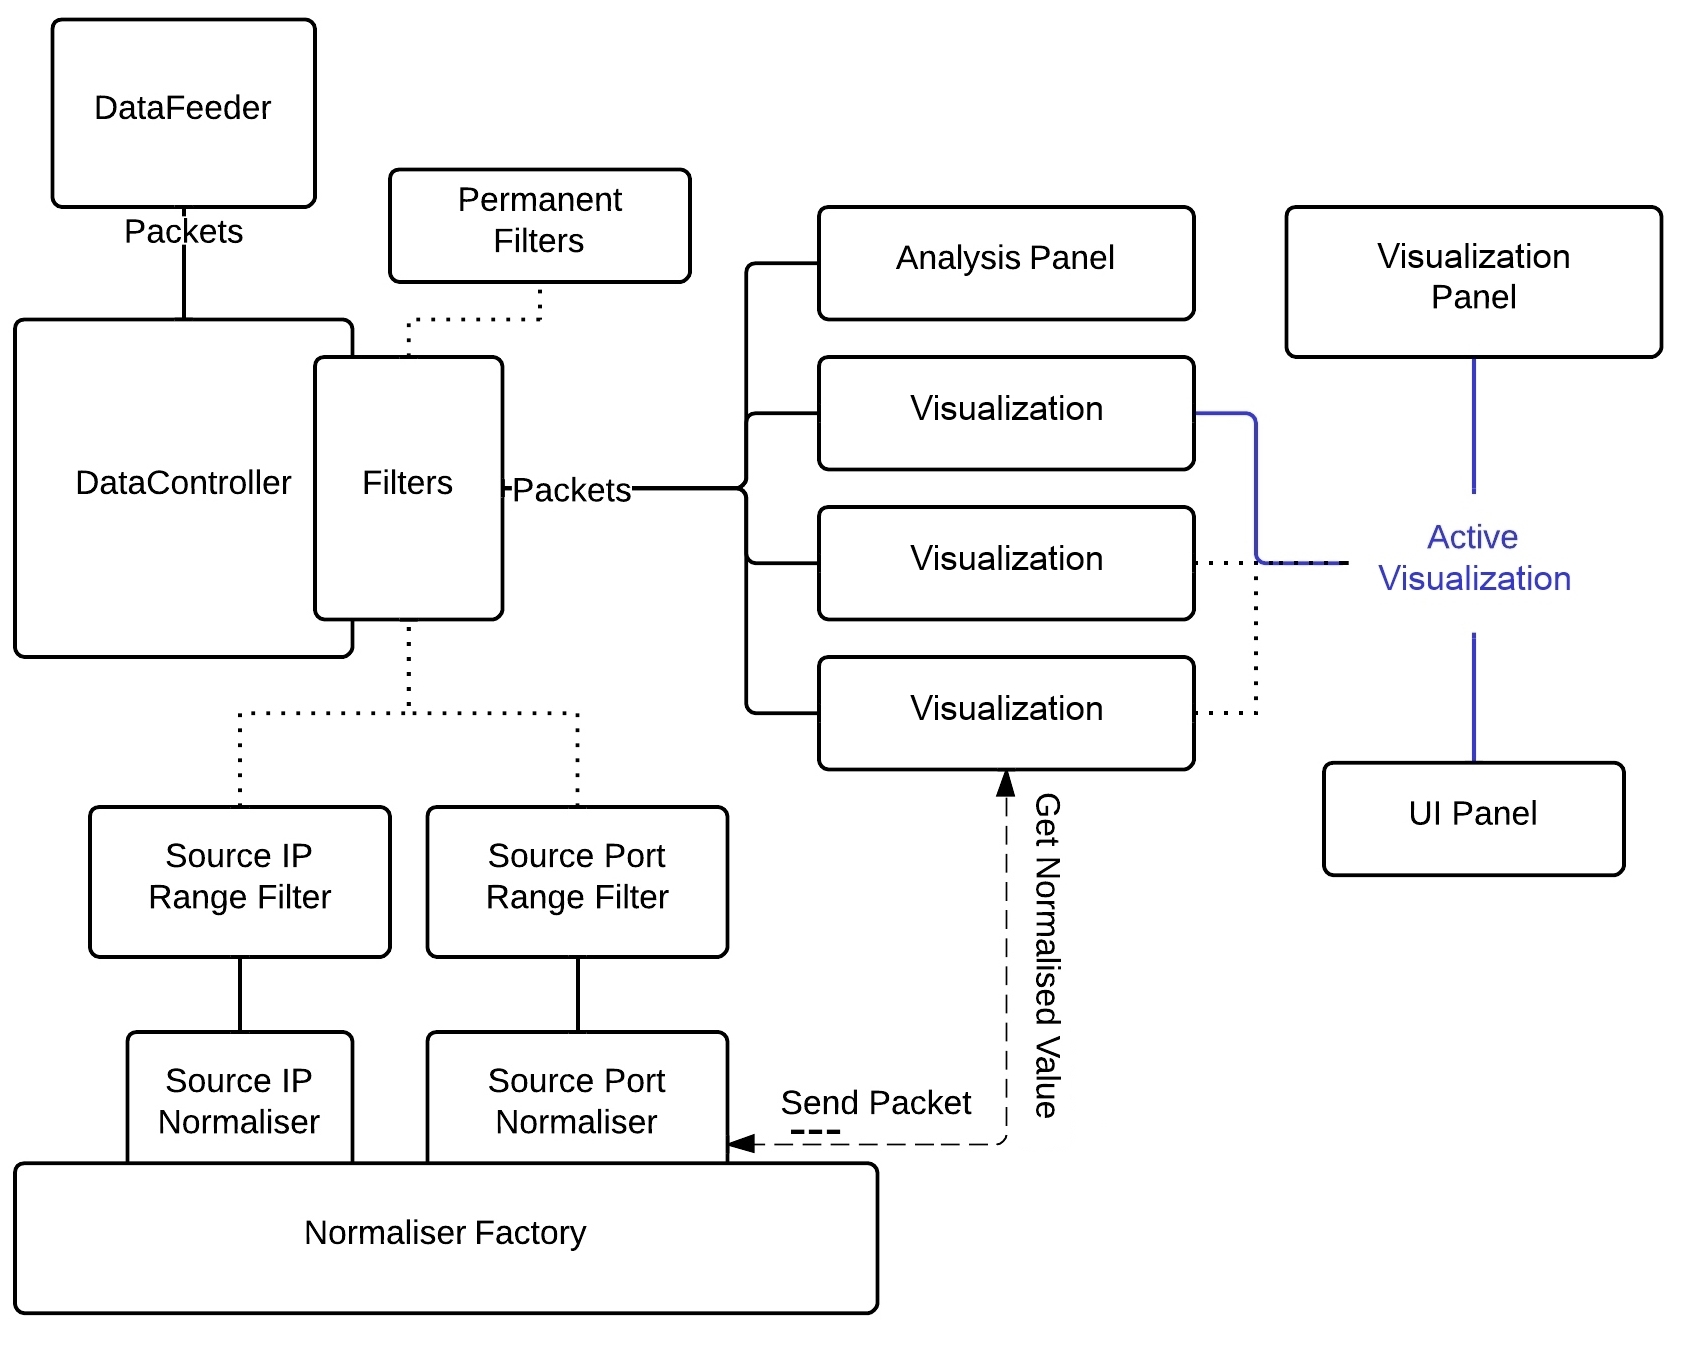
\includegraphics[width=\linewidth]{materials/architecture.jpg}

Filtering:
\textbf{High-level: What do filters do?}
The application supports two types of filters - filters that the user explicitly defines, and filters applied on-the-fly from within the visualisations.
Both types are applied to all visualisations and information displayed, and can be adjusted at any time without losing prior data.
The user has access to a variety of different filter controls.  First, there is a menu for filtering by transit protocol. By default, all protocols are selected and therefore included. Protolcols are sorted into menus by protocol family, appearing in multiple places where appropriate. Second, there is a control to select the range of ports the application uses, which defaults to the maximum port range.  The source and destination ports can be set separately, enabling a user to view all data entering/exiting a port as desired.  Next, there are IP and MAC address filters.  These work on a blacklist/whitelist system, allowing a user to only view packets to or from a particular set of addresses, or ignore packets going to or from a different set.  This enables a user to, for instance, ignore traffic from sources they know are irrelevant or focus only on an address that is causing concern.
The second type of filter will be dealt with in more detail in sections 4.2 and 4.3.

Modularity: \textbf{[Make this better.]}
The application was designed to be very extensible.  Adding a new visualisation is simply a matter of adding it to the application's list of those available, which will cause it to be included and kept up-to-date as packets come in and are filtered.  The same is true for filters and normalisers.  \textbf{[wrong place:] }Adding a filter would result in its controls automatically being included in the right panel and all packets would then be filtered according to the criteria it specifies.  Adding a normaliser would cause it to be integrated with the Spinning Cube, Dataflow and Attribute Distribution visualisations.  Ths modularity extends even so far as data input.  If a class were written to accept packets from a different source, it would be trivial to switch the application to use this class.